\section{Exploitation Patterns}
\frame{\sectionpage}

\begin{frame}{Exploitation of Vulnerabilities in V8 // Chromium}
    \begin{enumerate}
        \item Use the vulnerability to trick V8 into creating an array with an incorrect length. 
        \item Use the corrupted objects to generative out-of-bounds access primitives on the JS Heap. 
        \item With OOB access, create the \textit{addrof} and \textit{fakeobj} primitives for manipulating JS objects. 
        \item Use the \textit{addrof} and \textit{fakeobj} to create arbitrary read and arbitrary write functions.
        \item Gain code execution with the read/write functions via one of
            \begin{itemize}
                \item Overwriting RWX memory from WebAssembly code.
                \item Embed shellcode in JIT-compiled floating point instructions.
                \item Stack pivot from the pointer cage into a version specific ROP chain. 
            \end{itemize}
        \item Pop calculators!
    \end{enumerate}
    \break
    An example PoC showing these can be found below, a full analysis can be found \href{https://faraz.faith/2021-01-07-cve-2020-16040-analysis/}{\color{pink}here}.
    \break
    \href{https://www.exploit-db.com/exploits/49745}{\color{pink}{https://www.exploit-db.com/exploits/49745}}
    \note{
        \begin{itemize}
            \item All vulnerabilities discussed here can be exploited in scripts to 99\%+ certainty.
            \item Unlike in binary exploitation problems, there are no size restrictions, byte restrictions, cache coherenecy, etc.
            \item Exploitation is entirely stateless, and can be restarted easily.
            \item The biggest problem in V8 exploitation is garbage collection, the "invisible" hand that moves memory addresses around.
            \item Exploit patterns evolve rapidly overtime, techniques from even a few months ago are invalid now.
        \end{itemize}
    }
\end{frame}

\begin{frame}{Part 1 -- Create an Array with Incorrect Length}
    \begin{columns}
        \begin{column}{0.5\textwidth}
            \usemintedstyle{vim}
            \inputminted{js}{code/exploit-1.tex}
        \end{column}
        \begin{column}{0.5\textwidth}
            \usemintedstyle{vim}
            \inputminted{js}{code/exploit-1-1.tex}
            \begin{itemize}
                \item This is the implementation of CVE-2020-16040.
                \item It creates an array "arr" with length = -1. 
                \item However, V8 has not adjusted the backing store for that array, leading to OOB access on the JS Heap.
            \end{itemize}
        \end{column}
    \end{columns}
    \note{
        \begin{itemize}
            \item You can't write to the length property directly because it will cause V8 to allocate more memory.
            \item If you trick the engine with an OOB write, V8 will assume the array is longer but won't allocate more memory. 
            \item This vulnerability is not really a type confusion, but the underlying issue does lie within Turbofan.
            \item Turbofan mathematically (and incorrectly) proves that the function 'vuln' can never allocate an array with nonzero length.
            \item The for loop triggers Turbofan's JIT compilation of the 'vuln' function, and insufficent deoptimizations occur in the vuln(false) function call. 
        \end{itemize}
    }
\end{frame}

\begin{frame}{Part 2 -- Creating OOB access on the JS Heap}
    \begin{columns}
        \begin{column}{0.5\textwidth}
            \usemintedstyle{vim}
            \inputminted[]{js}{code/exploit-2.tex}
            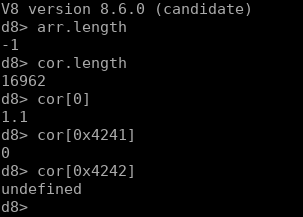
\includegraphics[width=\textwidth]{images/v8-length-screenshot.png}
        \end{column}
        \begin{column}{0.5\textwidth}
            \begin{itemize}
                \item In this snippet, "offset" represents the distance in memory from "arr" to "cor" on the JS heap. 
                \item This snippet uses out-of-bounds access via "arr" to modify the metadata of "cor".
                \item This overwrites the length of "cor" to be 0x4242, which grants OOB access on the JS Heap. 
            \end{itemize}
        \end{column}
    \end{columns}
    \note{
        \begin{itemize}
            \item This part of the exploit isn't really necessary, since the array length of 'arr' is already corrupted. 
            \item However, it nicely illustrates the OOB access. 
            \item Note that if garbage collection happens unexpectedly, the OOB access can get messed up! 
        \end{itemize}
    }
\end{frame}

\begin{frame}{Part 3 -- Create the \textit{addrof} and \textit{fakeobj} primitives}
    \begin{columns}
        \begin{column}{0.5\textwidth}
            \usemintedstyle{vim}
            \inputminted[]{js}{code/exploit-3.tex}
        \end{column}
        \begin{column}{0.5\textwidth}
            \begin{itemize}
                \item "addrof" is a function this takes in an arbitrary JS object \textit{k}. Using "arr" OOB write, insert \textit{k} into "cor" (replacing 1.1). Then, read the object from "cor". This will read the pointer to \textit{k} as it were a float. 
                \item "fakeobj" is the opposite of addrof; rather than leak pointers to the JS runtime, it allows the JS runtime to insert arbitrary values that V8 will interpret as a pointer. 
            \end{itemize}
        \end{column}
    \end{columns}
    \note{
        \begin{itemize}
            \item 'addrof' and 'fakeobj' originally come from a phrack article written by Samuel GroB, former project-zero now the head of the V8 security team.
            \item The premise here is that OOB access by one object doesn't update the HiddenClass of another. So if one uses 'arr' to write into 'cor'. The engine still thinks that 'cor' is an Array of floating point numbers. Thus, the memory address of the object will be returned as a floating point value. 
            \item Note, this would NOT work if the pointer cage was in place! Since valid pointers do not exist on the heap (unless they point to other things also on the heap)!
            \item fakeobj tricks the V8 engine into thinking some blob of memory is actually a JavaScript object. It is helpful for gaining arbitrary writes. 
        \end{itemize}
    }
\end{frame}

\begin{frame}{Part 4 -- Create Arbitrary Read and Arbitrary Write Functions}
    \begin{columns}
        \begin{column}{0.5\textwidth}
            \usemintedstyle{vim}
            \inputminted[]{js}{code/exploit-4.tex}
        \end{column}
        \begin{column}{0.5\textwidth}
            \begin{itemize}
                \item The first three lines:
                    \begin{itemize}
                        \item Read the HiddenClass for the built-in Array type using OOB access
                        \item Create a legitimate object "arr2" which contains the array map 
                        \item Create an illegitimate object "fake" using the array contents of "arr2" 
                    \end{itemize}
                \item For both functions, arr2[1] points to the fake's \textit{backing store}, that is, the memory location where the contents of "fake" are stored. 
            \end{itemize}
        \end{column}
    \end{columns}
    \note{
        \begin{itemize}
            \item In this version of V8, the metadata of a JSArray object has a pointer inside of its metadata called the "backing store". 
            \item This "backing store" pointer points to a memory region that contains enough space to contain the elements of the array.
            \item However, if the "backing store" pointer were to become corrupted by an attacker, then an attacker can use that array in JS to obtain arbitrary read and write locations.
            \item To do this, leak the base address of the JSArray object using `addrof`. Then set its backing store to the argument `addr`, then, read/write to the address and return its value. 
            \item In practice, its best to restore the original backing store of the Array, otherwise triggering garbage collection can crash the engine. 
        \end{itemize}
    }
\end{frame}

\begin{frame}{Part 5 -- Allocate a RWX Page using WebAssembly}
    \usemintedstyle{vim}
    \inputminted[]{js}{code/exploit-5.tex}
    \begin{center}
        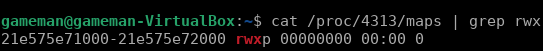
\includegraphics[width=0.8\textwidth]{images/v8-memory-rwx.png}
    \end{center}
    \break
    \begin{itemize}
        \item In this version of Chrome, WebAssembly functions will allocate RWX memory by default.
        \item In late 2021, V8 started toggling WASM code pages between writable and executable. 
        \item Recently, V8 developers introduced an additional sandbox on the JS Heap.
    \end{itemize}
    \note{
        \begin{itemize}
            \item WebAssembly is special type of assembly code generated by compiled languages to run in a browser context.
            \item In this version of Chrome, webassembly code lives in directly accesible RWX memory. 
            \item This RWX memory didn't see any kind of additional protections until 2021!
            \item This illustrates how while bugs in V8 haven't changed much, in reality the exploit patterns have become significantly harder.
        \end{itemize}
    }
\end{frame} 

\begin{frame}{Part 6 -- Overwrite the contents of the RWX pages}
    \begin{columns}
        \begin{column}{0.5\textwidth}
            \usemintedstyle{vim}
            \inputminted[]{js}{code/exploit-6.tex}
        \end{column}
        \begin{column}{0.5\textwidth}
            \begin{itemize}
                \item Leak the address of the WebAssembly instance using \textit{addrof}.
                \item A pointer to the RWX page will be at offset 0x68 from the leaked address. 
                \item Dereference that pointer using \textit{arbread}. 
                \item Copy some shellcode into the body of that rwx page and pop a calc!
            \end{itemize}
        \end{column}
    \end{columns}
    \note{
        \begin{itemize}
            \item Since the V8 exploit destabilizes the renderer process in the browser, exploit engineering beyond a PoC largely involves stabilizing the browser. 
            \item Note that normal shellcode here won't work in a browser because of the seccomp-bpf sandbox.
            \item The renderer is restricted to a small number of system calls it is allowed to make, execve is not one of them.
            \item However, running the exploit in d8, the command line version of V8, will work fine. 
        \end{itemize}
    }
\end{frame}

\begin{frame}{Part 7 -- Pop a calc!}
    \centering
        \Huge\bfseries
    \textcolor{yellow}{Calculator time!}
    \note{
        \begin{itemize}
            \item If running in Chrome on Linux, the "--no-sandbox" flag should be passed on the command line.
            \item To verify the sandbox is off, use "chrome://sandbox" in the URL.
            \item The exploit needs to be packaged as an HTML document to work properly.
            \item Chrome versions and V8 versions are directly correlated. V8 9.2 -> Chrome 92.
            \item Google publishes all commits to V8 and Chromium via CI/CD. One can freely download these and test on.
        \end{itemize}
    }
\end{frame}